\chapter {绪论}
\label{ch1}

\section{研究背景}

在现在社会,人们和移动设备的关系越来越密切,衣食住行几乎都离不开手机。
每天,人们只需要打开手机上的应用,就可以完成几乎所有的生活需求,
从出行打车到在线订餐,从网上购物到房屋租赁。
移动应用已经深入到人们生活的方方面面。
以移动系统Android为例,根据著名网站statista的统计~\cite{GoogleP55:online}显示,Android官方应用平台 Google Play Store在2009年12月至2018年6月期间的应用数量变化如~\autoref{fig:app_number}所示。
Google Play Store于2008年8月上线,截止2018年3月,在Google Play Store 上架的应用已经超过330 万。
这个数字在2013年7月才刚刚突破100万。这也从一个侧面反映出最近几年移动应用迅猛的增长趋势。

 \begin{figure*}[hb]
	\centering
	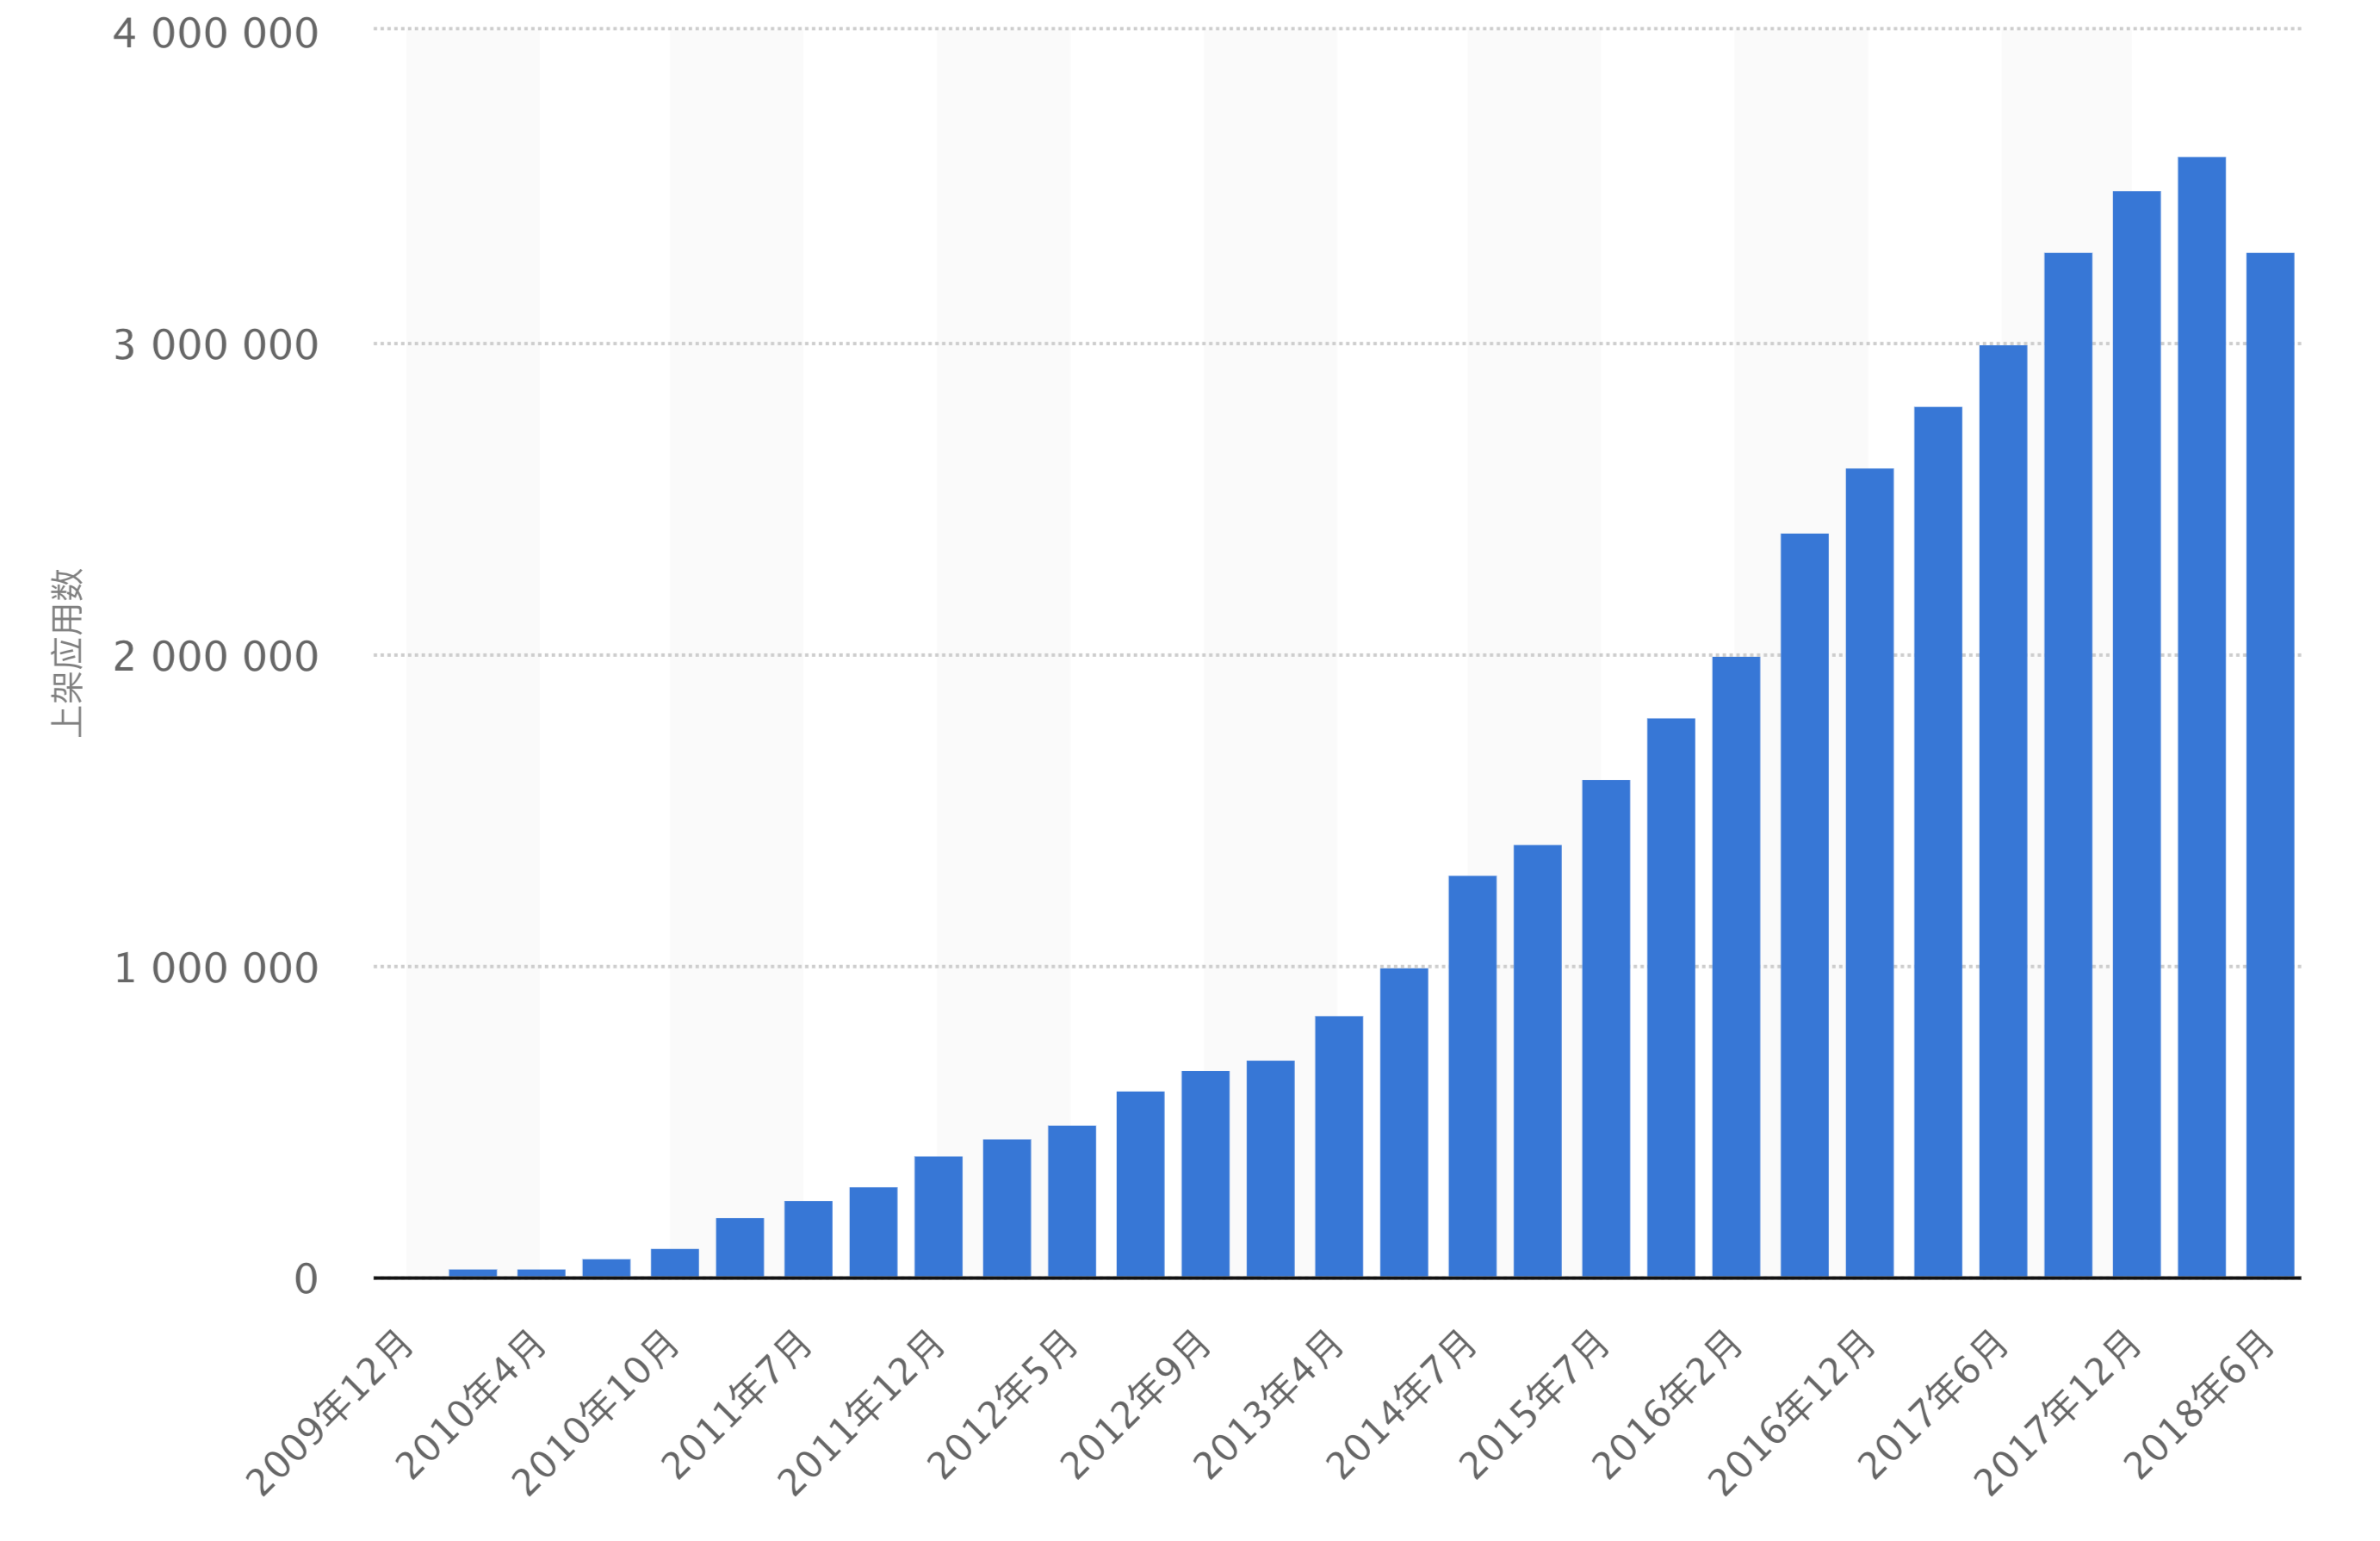
\includegraphics[width=\textwidth]{./Figures/app-numbers.png}
	\caption{Google Play Store上架的应用总数的变化趋势}
	\label{fig:app_number}
\end{figure*}


正因为移动应用迅猛的增长趋势,学术界和工业届的相关人员开始研究如何通过技术手段分析移动应用的代码内容,了解应用本身的运行时行为,进行相关学术研究和工业生产。
利用程序分析技术,研究人员对应用程序的项目相关源代码、配置文件或者二进制分发文件进行分析,监控程序的运行时行为,总结出应用程序相关特征。
结合具体应用场景,我们对这些特征进行归纳总结出相关规律,应用在应用分析、安全风险以及质量保障等领域,进一步提升应用程序的易用性、安全性和可靠性。

根据分析过程中是否需要运行目标程序,我们可以将这些技术手段分为静态分析技术和动态分析技术。
如果分析过程不依赖于目标程序的运行,这种分析技术称为静态分析技术,反之则为动态分析技术。
静态分析技术通常以二进制程序文件作为研究主体,结合相应的控制流分析、数据流分析技术、指针分析以及程序依赖分析,得出应用程序过程内的控制依赖和数据依赖(两者统称为程序依赖);
根据程序方法内相关函数/方法\eat{在Java语言中,函数称为方法。在本文中,两者可以相互替换,不做区分。}调用,可以得到函数调用图、UML类图和序列图;
我们将程序依赖数据和函数调用图相结合,可以进一步得到过程间程序依赖~\cite{stafford2000formal},帮助研究人员了解程序整体层面的业务间的依赖关系,进行污点传播分析。
相反的,动态分析技术依赖目标程序的运行,通过修改目标程序的运行文件,搭建目标程序的运行环境,记录程序运行过程中相关操作信息,监控目标程序在运行过程中的状态变迁或指标变化,
进而得出程序在运行过程中的行为特定,帮助研究人员进行程序安全性分析,提升程序的质量可靠性。

但是,上述两种技术各有各的优劣。
静态分析技术有着较为扎实的理论基础,分析结果精确可靠,覆盖范围全面。
但是,静态分析技术在枚举所有情况时,往往会遇到状态爆炸的问题,具体实验效果受到实验运行环境的硬件条件和算法实现程度的限制。
而且,静态分析技术分析的问题依赖于外部环境(用户实时操作序列、手机所处环境因素,如温度等),分析得到的结果并不是非常准确。
动态分析技术却能解决这个问题,通过对程序运行状态的监控,研究人员可以了解程序的运行行为,掌握程序的安全性信息和可靠性信息。
但是,动态分析技术的缺点也非常明显:动态运行环境的搭建往往要设计到相关系统的源代码,构建系统的时间成本大,技术要求高。
另外,动态分析技术的分析结果往往只针对一次程序的运行过程,无法直接推广到其他运行情况。

Android应用程序的特性(例如,基于事件驱动的基础架构、面向组件的开发方式、高度依赖回调函数和多线程交互等)使得传统分析工具无法直接应用在Android程序上,对研究人员了解Android应用程序执行细节造成了一定的困扰。
为了解决这个问题,本文提出了一种静动态相结合的技术方案,通过程序源代码和运行环境进行预处理,获得程序的运行时信息,进而还原出Android应用程序的动态函数调用图。
在调用图中,除了方法调用关系,我们还提供了方法对象、方法间触发关系等信息,可以帮助研究人员补全函数关系,较为全面地了解应用程序运行时的状态变化。




\section{Android分析技术}

通常的,软件分析技术主要分为静态分析技术和动态分析技术两类。

\subsection{静态分析技术}

在不执行应用程序的情况下,静态分析技术通过对应用程序的源代码或者执行文件进行控制流分析和数据流分析,进而推断应用程序在运行过程中可能产生的行为。
这方面相关工具包括Soot~\cite{vallee1999soot}、FlowDroid~\cite{arzt2014flowdroid}、AmanDroid~\cite{AmanDroid}、IccTa~\cite{iccta}、androguard~\cite{androguard:online}等。
Soot是传统的静态分析工具,其思路是将所有的Java字节码文件转化成一种中间语言Jimple,并在Jimple的基础上进行常规的控制流分析、数据流分析,理论上适用于所有可以在Java虚拟机上运行的语言(例如Scala、Groovy等等)的分析。
由于Android程序本身的字节码Davlik和Java字节码在格式上保持一致,因此,Soot也支持Android应用程序的静态分析。
但是,Soot在分析过程中没有考虑一些Android的特性难免会出现一些问题。
为此,德国达姆施塔特工业大学的Steven Arzt等人在Soot的基础上考虑Android程序中Activity的生命周期特性,推出了一个针对Android的静态分析工具FlowDroid,可以做到上下文、路径、对象、字段等层面上的敏感。
FlowDroid通过定义数据源点和数据泄漏点,在Android应用生命周期的基础上,可以实现数据流敏感的污点分析。
但其不足之处在于缺少跨组件通信的分析不考虑多线程调用问题。
在FlowDroid基础上,卢森堡大学的Li Li等人推出了IccTA,利用跨组件通信分析工具IC3提取跨组件通信(Inter-Component Communication, ICC)的方法调用,并结合AndroidManifest.xml文件定义的Intent Filter信息,连接ICC两端的组件,克服了FlowDroid因缺少跨组件通信而导致的数据流上的缺失。
因为它是构建在FlowDroid之上的一个探测敏感信息泄露的,所以受限于FlowDroid的局限性。

Yang等人~\cite{yang2015static},利用静态分析技术,并将回调函数添加到控制流图(调用图)中,形成了回调控制流图(Callback control-flow gragh)。
实验结果显示,Yang的工作比Gator~\cite{rountev2014static}在控件监听器绑定上得到了更为准确结果。
法国和意大利的学者~\cite{payet2012static}通过对Java字节码静态分析器Julia进行扩展,使得其支持对 Android 应用程序的静态分析;
他们通过改写 Android 库中 Activity、LayoutInflater 等类的代码逻辑,规避了Android系统分析常见难点(如程序的事件机制,基于反射的视图加载等),
实现了包括死代码检查、空指针检查在内的7种静态分析技术。



%由此可见,静态分析工具在分析过程中虽然可以对应用程序进行较为全面的分析,覆盖应用程序的所有代码,但由于缺少和程序执行过程相关的部分必要信息(应用程序的执行序列、和设备所处环境相关的传感器(如GPS、温度等)信息等),可能导致部分情况下分析结果的不精确。为了解决这一问题,研究人员提出了动态分析技术。


\subsection{动态分析技术}

% 为了解决这一问题,研究人员提出了动态分析技术。
和静态分析技术相对应,动态分析技术通过执行应用程序,获取程序运行过程的相关信息,从而实现对应的研究目的。
动态分析技术往往需要对运行环境做适当的修改或者调用特殊的系统接口,记录应用程序运行过程的关键信息,结合数据流追踪等技术,已记录应用程序的运行时行为。
这方面的工作代表包括TaintDroid ~\cite{chun2014taintdroid}、DroidBox~\cite{droidbox:online}、TraceDroid~\cite{van2013dynamic}、DroidScope~\cite{droidscope}等。
Enck等人提出的TaintDroid,是一个高效的系统级的动态污点跟踪和分析系统。它通过修改Dalvik虚拟机,利用动态污点分析技术实时监控敏感数据的生成、传播和泄露,实现了变量层面、方法层面、文件层面的数据追踪。
此外,TaintDroid还支持跨进程通信(IPC)层面上的污点分析,因此可以精确分析出应用程序从消费者手机上获取和发布隐私信息的完整传播过程。
TaintDroid提供了较为完备的数据流分析技术,但是不支持控制流追踪,无法给出相关语句的执行路径。
DroidBox在TaintDroid基础上,对Android Framework的部分API做了修改,可以记录一些开发人员感兴趣的API(例如文件读写、网络请求、SMS服务等)的调用,并提供分析结果的可视化。
同时,DroidBox还实现了应用程序的自动安装和执行,弥补了TaintDroid在软件测试自动化方面的不足。
和TaintDroid不同,TraceDroid采用的是另一种思路,利用字节码插装技术AspectJ,使得方法在执行时输出相应的日志信息。根据这些信息TraceDroid可以还原函数调用图,得到分析结果。
由于Aspect在进行字节码编织时引入的新的方法会导致生成源APK文件中的方法总数超过65536~\cite{Configur27},进而使得APK文件无法成功构建,因此该方案存在不稳定的情况。

另外,研究人员还用动态分析技术查找Android应用程序在运行时性能瓶颈。Android官方性能检测工具SimplePref~\cite{simpleperf:online}就是其中的一个代表。
SimplePref利用了Linux提供的系统接口pref\_event\_open,定时获取到性能监视单元的相关信息(例如cpu周期数、执行的指令数、缓存失效次数等)。
利用这些信息,SimplePref可以得到对应时刻的CPU状态,还原出各个方法的执行时间和对应的执行路径。
根据方法执行时间的长短和对应的执行路径,开发人员可以发现程序的性能瓶颈,进而通过对程序代码做出调整,提升程序的运行性能。
但是,该方法受到系统接口回调周期的影响,过于频繁的调度周期会使系统产生过大的开销,影响原有程序的执行;反之,则会丢失部分方法的执行信息。
而且,Android程序关心的性能瓶颈一般都位于主线程,而SimplePref会输出所有线程的执行信息,实际开销较大。
为此,Uber的Nanoscope~\cite{ubernanoscope:online}采用追踪(Trace)技术在定制化的系统Nanoscope OS中运行,在虚拟机解释执行目标方法前后输出相关Trace日志,进而得到性能报告。
相比SimplePref,Nanoscope只输出主线程相关的方法数据信息,大大减低了性能上的开销。
但是,nanoscope的局限性在于构建成本较高,需要配合特定的系统使用。


\begin{comment}

6.3.1 AASandbox 
In October 2010, Blasing et al. were the first to present a dynamic analysis platform for Android applications: AASandbox (Android Application Sandbox) [7]. It uses static analysis to scan software for malicious patterns and performs dynamic analysis to intervene and log low-level interactions with the system for further analysis by means of a loadable kernel module developed to obtain system call logs. AASandbox uses a system call footprinting approach for detecting suspicious applications. Unfortunately, there were no known Android malware samples available at the time to evaluate this technique. AASandbox seems to be unmaintained nowadays. Compared to AASandbox, TraceDroid is implemented on a higher abstraction layer, namely the Dalvik VM instead of the Linux kernel. This allows TraceDroid to retrieve great detail on executed Java components, while missing any native code execution paths. By using the strace utility, however, we obtain a similar overview of executed system calls. We already use analysis output to detect suspicious activity. 
6.3.2 TaintDroid 
Also in October 2010, Enck et al. presented TaintDroid: a modified Android OS keeping track of taint propagation at runtime to detect privacy leaks [26]. Over time, it has been adopted as a valuable addition by many subsequent research proposals which aim to perform dynamic analysis on Android applications. TaintDroid is implemented as a modification of the Dalvik VM and thus cannot track taint within native code. TaintDroid does not come with a set of scripts or applications to allow automated analysis and stimulation of unknown applications and is thus quite different compared to our TraceDroid platform. It does also not keep track of any specific method invocations. What we could do, however, is extending TraceDroid in such a way that it also keeps track of field operations, and use this data to implement taint tracking functionality as a post-processing plug-in. 
6.3.3 DroidBox DroidBox was developed by Patrik Lantz as part of Google Summer of Code (GSoC) 20113 . It combines TaintDroid with modifications of Android’s core libraries. The modified Android OS of DroidBox logs the following events during runtime of an application: • File read and write operations. • Cryptography API activity. • Opened network connections. • Outgoing network traffic. 3http://www.honeynet.org/node/744 78 • Information leaks through network, files or SMS messages (using TaintDroid). • Attempts to send SMS messages. • Phone calls that have been made. It also provides visualization of analysis results and automated app installation and execution. TraceDroid differs from DroidBox in that our implementation traces all method invocations, including those occurring within an application, while DroidBox looks only at a small subset of API calls of which the developers think are interesting. Our approach is beneficial, for example if malware authors use third-party cryptographic libraries instead of the hooked APIs to encrypt data. DroidBox operates on the core library level, while TraceDroid is integrated at the Dalvik bytecode interpreter. This makes TraceDroid a more suitable platform for detailed analysis of unknown applications. On top of that, our TraceDroid Analysis Platform performs a more fine-grained level of simulation techniques when compared with DroidBox. A second version of DroidBox was developed by Kun Yang as part of GSoC 2012 and introduces an APIMonitor that uses bytecode rewriting instead of core library modifications4 . While this is a good approach to overcome the need of continuously upgrading DroidBox to newer Android versions, rewriting applications breaks an app’s original signature which can easily be detected at runtime. Also, as with the first DroidBox release, the APIMonitor can only monitor core API calls which results in a less comprehensive set of traced method invocations than TraceDroid achieves. Since DroidBox was the first openly available dynamic analysis platform for Android, it has been used as a base system by many other dynamic analysis platforms including Andrubis, Mobile-Sandbox, and SandDroid. 6.3.4 Bouncer In February 2012, Google announced Bouncer [44]. It is stated that every application that is offered for download in the Google Play Store is run on Google’s cloud infrastructure and gets simulated as if it was running on an Android device. Since Bouncer is used to protect the Google Play Store from malicious applications, only sparse information was provided about its internal functioning. During Summercon in June 2012, however, Oberheide and Miller presented their efforts on dissecting Bouncer [? ]. Using a C&C application that connects back to their local machine, they determined that Bouncer runs dynamic analysis on applications for 5 minutes. They could setup a connect-back shell to communicate with the application under investigation5 and were able to obtain more detailed information on the environment used by Bouncer to run analysis. In October 2012, Google introduced an application verification service. With the release of Android 4.2, the ACTION PACKAGE NEEDS VERIFICATION broadcast was introduced, used by the OS to verify newly installed applications and check them for known malware. During installation, th the app (including its package name and its SHA1 hash) and the device (its ID and IP address) to the Google cloud and requests a verification response. Although not confirmed, the Google cloud likely uses Bouncer results to make statements about the app’s safety. A study performed by Xuxian Jiang shows that only 193 of the 1260 malgenome samples were detected as malicious by this verification scheme, indicating a detection rate of only 15.32%6 6.3.5 Andrubis In June 2012, the International Secure Systems Lab released Andrubis: a dynamic analysis platform for Android applications [42]. Andrubis was the first to offer a publicly available web interface where users can submit Android applications for dynamic analysis. When analysis is finished, it generates a XML report containing a behavioral and static analysis footprint of the requested application. Its first release was based on DroidBox’s core library modifications and was built on top of Android 2.1. Andrubis was later updated to run under Android 2.3.4 and uses VMI to intercept system calls made by native code execution. With the integration of TraceDroid, Andrubis has become a very extensive dynamic analysis platform that does not only track taint propagation to detect privacy leaks, but also records invoked system calls and comprehensive Java method traces. Due to our collaboration efforts, Andrubis has adopted most of TraceDroid’s functionality. 6.3.6 DroidScope First presented in August 2012, DroidScope is a comprehensive dynamic binary instrumentation tool for Android based on VM introspection [72]. It reconstructs Dalvik instruction traces and this could, in theory, be used to obtain the same results as we currently obtain with TraceDroid. The key difference between TraceDroid and DroidScope, however, is the fact that DroidScope is bound to an emulator, while TraceDroid may run on actual hardware. Malicious applications can detect the use of an emulator and may decide not to start malicious activities in this scenario [55]. 6.3.7 AppsPlayground In February 2013, Rastogi et al. introduce AppsPlayground. Like previously discussed frameworks, AppsPlayground monitors taint propagation using TaintDroid, and traces specific Java API and system calls. Its main contribution is an improved monkey exerciser-like execution approach to explore application’s GUIs. The latter is something we would like to add to our TraceDroid Analysis Platform as well, as a mean to increase code coverage. 6.3.8 Mobile-Sandbox Mobile-Sandbox was released in March 2013 and is very similar to Andrubis in that it is based on DroidBox and uses TaintDroid to track taint propagation [64]. Instead of VMI to trace system calls, however, Mobile-Sandbox 6http://www.cs.ncsu.edu/faculty/jiang/appverify 80 uses a ported version of ltrace to trace native library invocations. This ltrace binary may be a valuable addition to our TraceDroid analysis platform. Like Andrubis, Mobile-Sandbox also allows users to submit Android applications for analysis via a web application. 6.3.9 CopperDroid Finally, in April 2013, Reina et al. introduced CopperDroid [58]. The mechanisms used in this system are similar to DroidScope as it also uses VMI to collect system call information about analyzed applications. Reina et al. argue, however, that CopperDroid points out how their system call-centric analysis and stimulation techniques can comprehensively expose Android malware behaviors. CopperDroid also comes with a web interface where users can submit unknown applications for analysis. 6.3.10 Closed frameworks A number of additional dynamic analysis platforms have been implemented and made available to the public via web applications. These frameworks, however, come with very little documentation on how they operate which makes it hard to make statements on any new approaches used by these implementations. It is likely that these platforms use (modified versions of) existing tools like DroidBox, TaintDroid and Androguard to complement their dynamic analysis engine. This is confirmed on SandDroid’s webpage, which states that it is powered by both DroidBox and Androguard7 . Example output reports of both ForeSafe8 and JoeSecurity9 suggest that these platforms use a combination of existing tools as well.

\end{comment}

\subsection{分析技术的应用}
\textbf{应用分类:}

Simapp~\cite{chen2015simapp}

mobile app tagging ~\cite{chen2016mobile}

WhyPer~\cite{pandita2013whyper}


\textbf{安全性分析:}


AppContext~\cite{yang2015appcontext}

AppIntent~\cite{yang2013appintent}

Socket~\cite{bu2017program}


\textbf{质量保障:}


Exception fault localization in Android applications~\cite{mirzaei2015exception}

machado2013mzoltar~\cite{machado2013mzoltar}


Fan~\cite{fan2018efficiently,fan2018large}

% 例如错误定位、自动化分析、profiling等

\section{本文的主要工作}

本文的主要研究工作包括以下:

1)	调研最近几年Android应用分析领域的静动态分析工具,了解各项工具的优劣以及相关的应用案例。

2)	提出并实现Android动态函数调用图构建系统,包含传统函数调用图的构建以及在此基础之上的多线程函数调用关系的构建。

3)	对上述系统设计对应的实验方案,评估对应的实验效果。

\section{本文的组织结构}

本文共分为六章,环绕着Android动态函数调用图构建系统的设计与实现展开,各章节内容如下:

第一章:主要介绍了本文的主要研究背景、主要工作内容以及研究意义,最后对本文的各章的内容做了阐述。

第二章:从Android的体系结构出发,并由此展开介绍了最近几年Android领域相关的静态分析技术和动态分析技术,以及这些技术在各自领域的运用,简单描述本文可能遇到的困难。

第三章:从系统功能、技术路线、技术选型、模块实现等若干方面介绍RunDroid的设计与实现。

第四章:从应用程序的构建效率、日志本身记录效率以及系统对程序运行的影响等三个方面设计并开展相关的测试实验。

第五章:将展示RunDroid系统生成的函数调用图的运行结果,并对函数调用图进行详细的阐述。

第六章:对本文工作进行总结,并对下一步工作进行展望。
